\documentclass[12pt]{article}

% Language setting
% Replace `english' with e.g. `spanish' to change the document language
\usepackage[T1]{fontenc}
\usepackage[english]{babel}

% Set page size and margins
% Replace `letterpaper' with`a4paper' for UK/EU standard size
\usepackage[a4paper,top=2.5cm,bottom=2.5cm,left=2cm,right=2cm,marginparwidth=1.75cm]{geometry}

% include graphics i.e images
\usepackage{graphicx}
\usepackage{fancyhdr} % headers
\usepackage[utf8]{inputenc}
\usepackage{gensymb}
\usepackage{subcaption}
\usepackage{array}
\usepackage{tabularx}
\usepackage{csvsimple}
\usepackage{titlesec}
\usepackage{lastpage}
\usepackage{pdfpages}
\usepackage{comment}
\usepackage{xcolor}
\usepackage{multirow}
\usepackage{verbatim}

\usepackage{lipsum}  

\setcounter{tocdepth}{1} % Exclude subsubsections from the table of contents


% include hyperlinks in the doc
\usepackage{hyperref}
%setup hyperref

\pagestyle{fancy}
\fancyhf{}
\rhead{\today}
\lhead{Marine Animal Tracking System}
\lfoot{PI - Wearable Sensing Device}
\rfoot{Page \thepage}
\renewcommand{\headrulewidth}{1pt}
\renewcommand{\footrulewidth}{1pt}



%------------------------------------------------------------------------------------------------
\title{PI}
\author{Benoit Schick}

\begin{document}

\begin{titlepage}
   \begin{center}
        \Huge
        Marine Animal Tracking System\\
        \Large 
        PI - Wearable Sensing Device 
            
        \vspace{1.5cm}
        \Large    
        Benoit Schick\\
        Warpelin Daryl\\
       	Jeyapalan Jeyapiragash\\
	Zweifel Robin
        
        \vspace{0.5cm}
        
        Supervisor:\\
        \vspace{0.1cm}
        Marco Mazza\\

        \vfill

        2024–2025 Academic Year, Spring Semester \\
        \vspace{1cm}
            
        \normalsize
        Multidisciplinary project\\
        \vspace{0.25cm}
        
	Master of science in Engineering 
        \vspace{0.25cm}
        
        \vspace{0.8cm}
            
        
\includegraphics[width=0.75\textwidth]{pictures/mse_logo.png}
        \vspace{1cm} 
        
   \end{center}
\end{titlepage}

\pagestyle{fancy}

\section{Hardware (Benoit Schick)}
\subsection{Défis et contraintes du système embarqué}

Le système développé dans ce projet doit fonctionner dans un environnement particulièrement contraignant, ce qui impose certains choix au niveau de l'architecture. 
\subsubsection{Isolement géographique}
L’une des contraintes fondamentales est la localisation des animaux suivis. Les espèces ciblées évoluent en haute mer, à des centaines voire des milliers de kilomètres de toute infrastructure terrestre. Dans ces zones, aucune technologie de communication classique n’est disponible : les réseaux cellulaires tels que le GSM, la 4G ou la 5G ne sont exploitables qu’à proximité des côtes, et les réseaux IoT longue portée comme LoRaWAN sont insuffisants pour cette application. \\
Dans ce contexte, la seule solution viable pour assurer une communication globale est la transmission par satellite. Deux technologies principales sont généralement utilisées dans ce type d’application :
\begin{itemize}
	\item \textbf{Le réseau Iridium} : Système qui repose sur une constellation de 66 satellites en orbite basse (LEO, ~780 km), offre une latence faible et une couverture totale.
	\item \textbf{Le réseau Argos} : Système satellite pour la localisation et la collecte de données désigné spécifiquement pour l'étude et la protection de l'environnement. Il est par exemple utilisé pour le suivi d'animaux marins et est largement adopté dans la communauté scientifique pour ce type d'application.  
\end{itemize}
Ces solutions permettent une communication globale mais introduisent des contraintes importantes en termes d’énergie et de disponibilité du signal.


\subsubsection{Contraintes du milieu marin}
Le milieu marin impose une contrainte majeure : l'eau de mer est un milieu extrêmement atténuant pour les ondes électromagnétiques utilisées pour la communication satellite. A quelques centimètres de profondeur seulement, tout signal est totalement absorbé et il est donc impossible de transmettre ou de recevoir quoi que ce soit lorsque l'animal est immergé, quelle que soit la puissance d'émission utillisée.\\
Cette contrainte impose un fonctionnement discontinu du système, alternant entre des phases d’immersion, où seules les mesures sont réalisées, et des phases de surface, où la communication est possible.

\subsubsection{Stockage temporaire}
L'impossibilité de transmission en continu des données exige d'intégrer une mémoire non volatile externe pour stocker temporairement l'ensemble des données acquises pendant les phases d'immersion (température, pression \footnote{Bien que fondamentale, la mesure de la pression a été abandonnée du à des contraintes budgétaires. Elle sera quand même évoquée dans ce rapport}, la position et horodatage des mesures). \\
Cette mémoire permet donc de gérer l’imprévisibilité des phases de surface, qui dépendent du comportement de l’animal et des conditions environnementales.

\subsubsection{Consommation}
Les conditions dans lequel le système va évoluer, introduit des contraintes importantes en termes de consommation énergétique. Les modules de communication, en particulier le GPS et le système satellite, figurent parmi les éléments les plus énergivores du système. \\
En effet, le module GPS nécessite une phase d’acquisition du signal satellite, qui peut devenir longue et coûteuse en énergie si les conditions de réception sont mauvaises ou si les fenêtres de surface sont très courtes. De même, le module de communication satellite présente des pics de consommation élevés lors de chaque tentative de transmission. \\
Ces contraintes sont aggravées par l’incertitude sur la durée et la fréquence des phases de surface, ce qui peut entraîner des activations répétées des modules de localisation et de communication, augmentant encore la consommation globale du système. \\

Or l’autonomie du système constitue un paramètre critique, car elle détermine la durée d’exploitation du dispositif ainsi que la capacité à le récupérer grâce au module GPS, chargé de transmettre la position du boîtier. Une stratégie de gestion énergétique est donc nécessaire afin de limiter le temps d'activation des modules GPS+satellite et maximiser le temps passé en mode low-power. Le système devra donc reposer sur une logique événementielle, dans laquelle les modules GPS et satellite ne sont activés que lorsque les conditions sont favorables, c’est-à-dire lors des phases de surface.


\subsection{Spécifications}

Le comportement de l’animal joue un rôle déterminant dans le dimensionnement du système. En effet, lorsqu’il est immergé, toute communication satellite est impossible. Le dispositif doit donc exploiter les phases de surface, durant lesquelles l’animal doit rester suffisamment longtemps pour permettre l’acquisition d’une position GPS ainsi que la transmission des données via le module satellite. La profondeur de plongée constitue également un paramètre critique, car elle impose des contraintes mécaniques importantes, notamment en raison de la pression exercée sur le boîtier. \\
Après comparaison avec d’autres espèces (cf. tableau), le choix s’est porté sur la tortue marine. Ce choix repose principalement sur ses phases de surface relativement longues et régulières, qui facilitent l’établissement d’une connexion satellite fiable et limitent les activations inutiles des modules de communication et de localisation. Cela permet ainsi de réduire la consommation énergétique du système tout en simplifiant certaines contraintes mécaniques.\\

L’autonomie représente un autre enjeu majeur. Le système doit être capable de fonctionner sur une longue durée afin de collecter un volume de données suffisant, tout en permettant idéalement la récupération du dispositif en fin de mission afin de limiter son impact environnemental. Cela implique une gestion optimisée de l’énergie, notamment en réduisant l’utilisation des modules les plus énergivores.\\

% Enfin, l’environnement d’utilisation impose des contraintes fortes en termes de communication. En raison de l’éloignement des infrastructures terrestres, les solutions classiques (GSM, LoRa, etc.) ne sont pas exploitables. L’utilisation d’une liaison satellite est donc indispensable pour assurer la transmission des données sur de longues distances.

\noindent Voici un résumé des spécifications prises en compte pour la partie Hardware du projet :

\begin{itemize}
    \item \textbf{Communication} : Transmission des données via un réseau satellite.
    \item \textbf{Localisation} : Acquisition de la position GPS du dispositif afin de permettre sa localisation et sa récupération
    \item \textbf{Stockage} : Utilisation d'une mémoire non volatile permettant l’enregistrement des données durant les phases d’immersion.
    \item \textbf{Autonomie} : Fonctionnement sur batterie avec un objectif d’autonomie d’environ un mois, reposant sur une optimisation de la consommation (modes low power, activation événementielle des modules).
    \item \textbf{Capteurs} : Mesure de la température de l'eau et de la profondeur (via un capteur de pression) en fonction de la position, afin de constituer une base de données exploitable pour permettre de suivre l'évolution thermiques des océans dans le cadre du réchauffement climatique.  
\end{itemize}


\subsection{Architecture générale} 
La partie électronique doit assurer de manière autonome la localisation de l’animal, l’acquisition de données environnementales, le stockage temporaire des mesures ainsi que leur transmission vers une infrastructure terrestre via un lien satellite. L’ensemble de ces fonctions doit être garanti dans des conditions environnementales extrêmes (pression, salinité, immersion), tout en maintenant une autonomie énergétique suffisante.

\begin{figure}[h!]
	\centering
	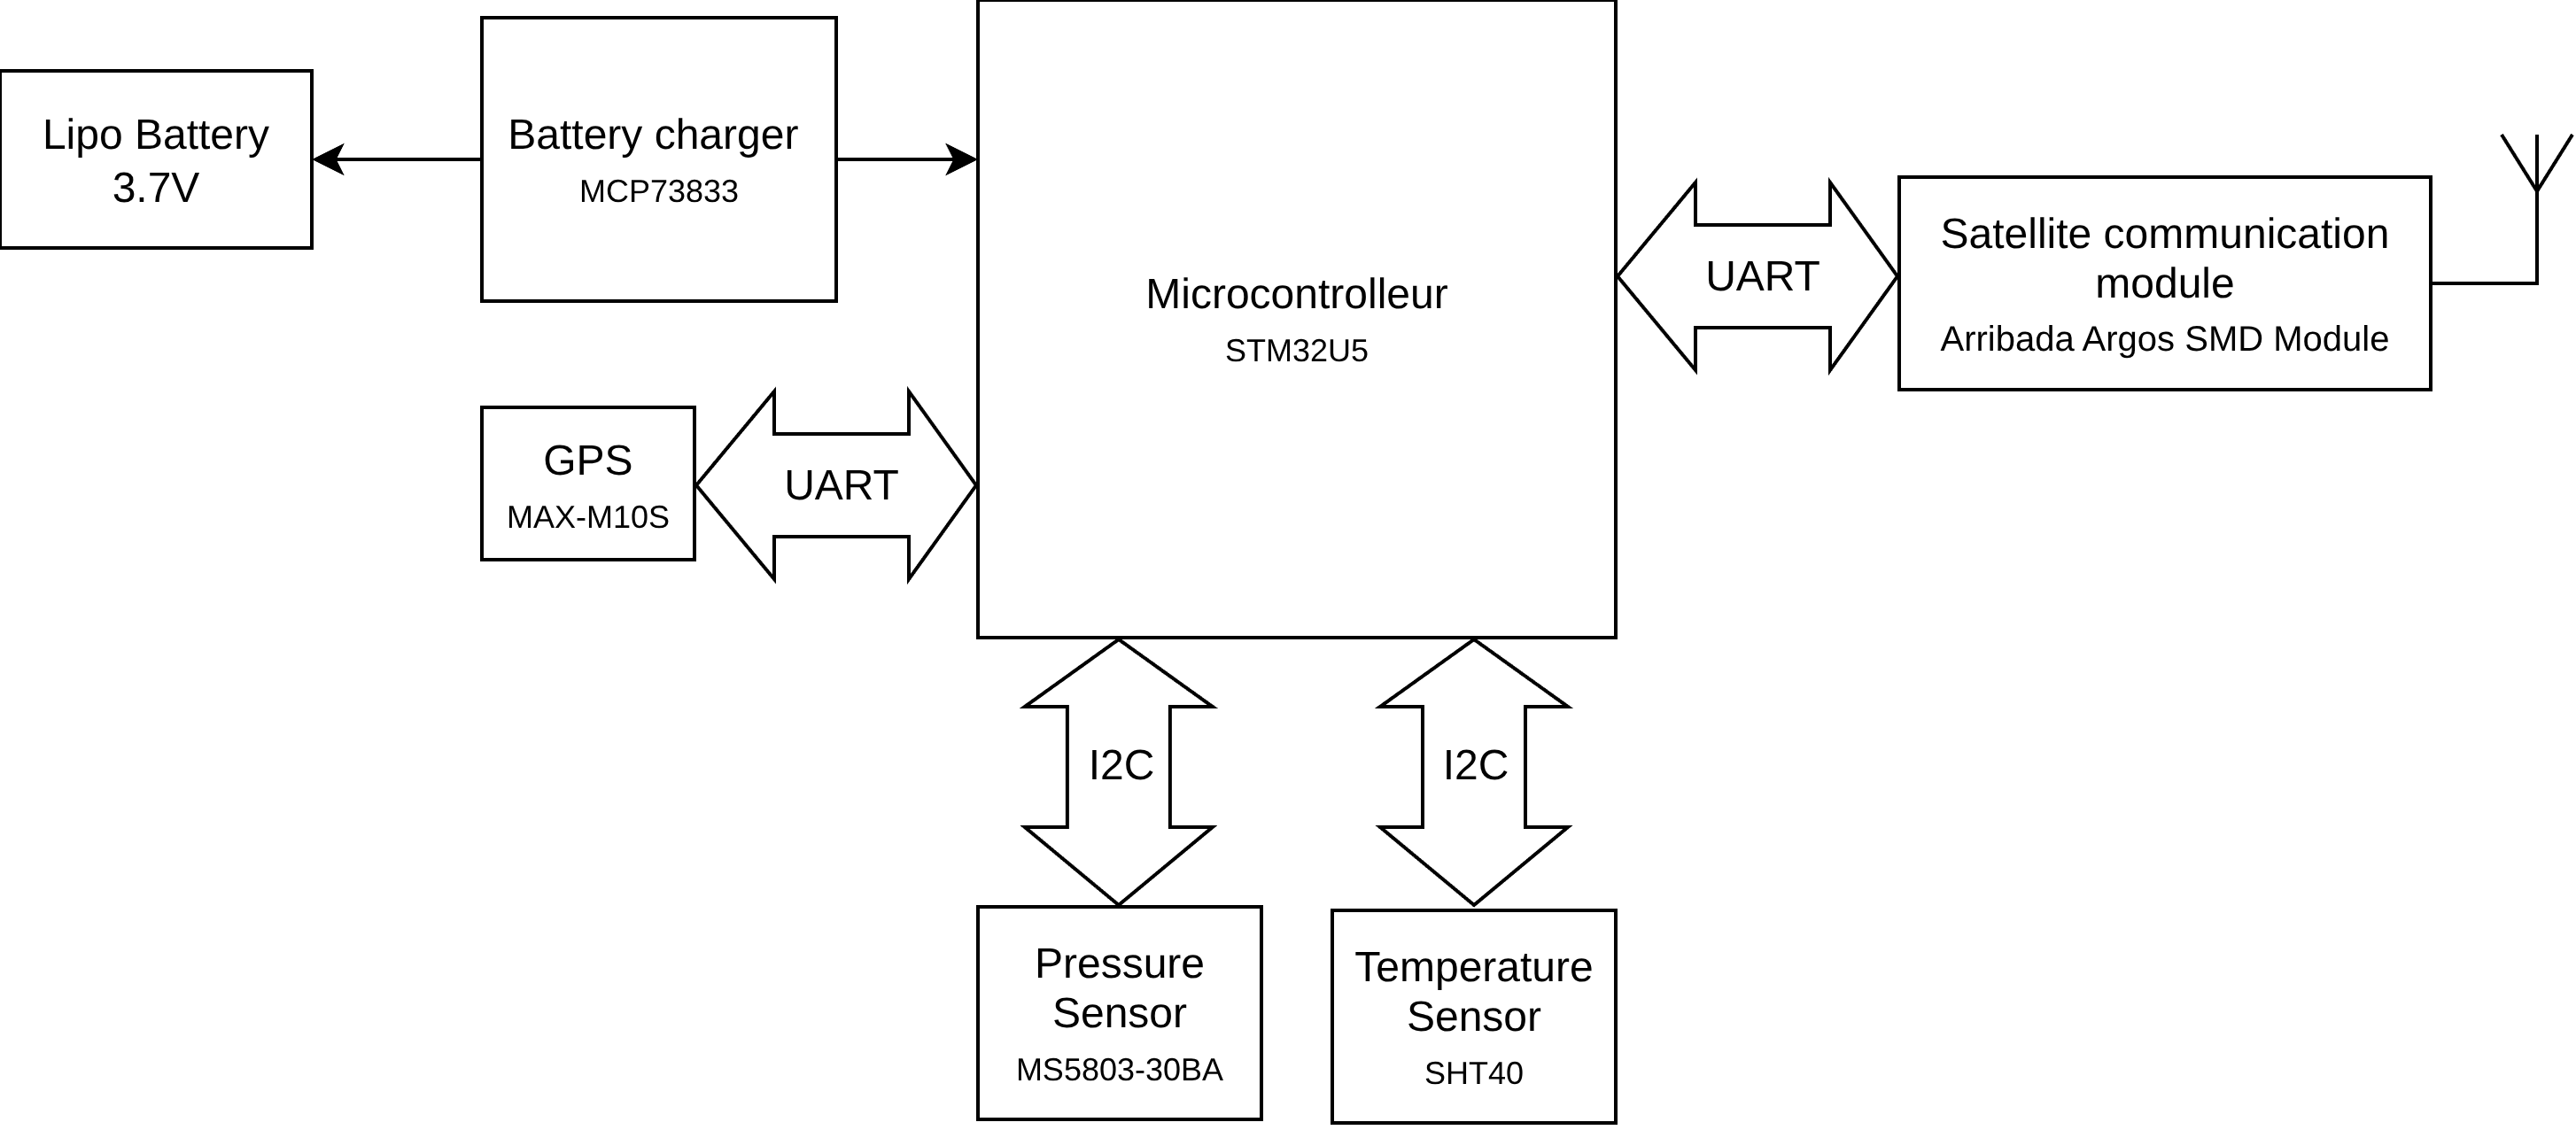
\includegraphics[width=\linewidth]{pictures/schema_bloc.png}	
	\caption{Schéma bloc de la partie Hardware}
	\label{fig:schema_bloc}
\end{figure}

L’architecture du système s’articule autour d’un microcontrôleur STM32U5 basé sur un coeur ARM Cortex-M33. Ce composant a été retenu pour sa très faible consommation (jusqu’à 160 nA en mode low power), sa compatibilité avec Zephyr RTOS facilitant le développement logiciel, ainsi que la présence de multiples modes low-power (7 modes) permettant d’adapter le compromis entre consommation, disponibilité des périphériques et sources de wakeup. Il intègre également un large éventail d’interfaces de communication (I2C, SPI, UART, USB), assurant l’interconnexion avec les différents modules du système. \\

L’alimentation repose sur une batterie Lithium-Polymère (LiPo) 1S d’une capacité de 10 Ah. Ce choix s’explique par sa forte densité énergétique, permettant de optimiser l’énergie stockée tout en réduisant la masse et le volume (Fig. \ref{fig:densite_bat}), ce qui constitue un critère essentiel pour une application embarquée sur animal. Néanmoins, ce type de batterie impose des contraintes strictes en termes de sécurité et d'utilisation. \\
La gestion de la charge est assurée par le circuit MCP73833, qui intègre les protections nécessaires contre la surcharge et la décharge excessive. Dans cette phase de prototypage, la recharge s’effectue via une interface USB-C. À terme, une solution de récupération d’énergie est envisagée, basée sur un générateur entraîné par une hélice mise en rotation par les déplacements de l’animal.

\begin{figure}[h!]
	\centering
	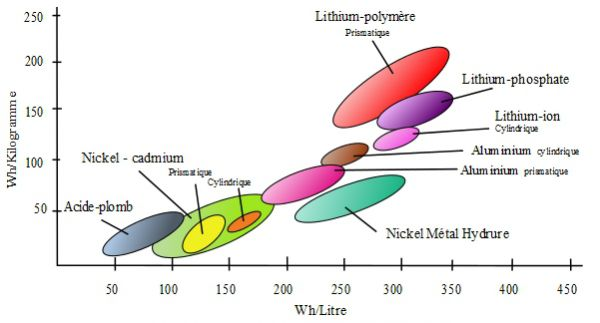
\includegraphics[width=0.5\linewidth]{pictures/densite_energie_batteries.jpg}	
	\caption{Densité d'énergie selon le type de batterie}
	\label{fig:densite_bat}
\end{figure}

La localisation est assurée par le module GPS MAX-M10S, sélectionné pour son faible niveau de consommation (environ 25mW en mode tracking continu), particulièrement adapté aux systèmes sur batterie. La communication avec le microcontrôleur s’effectue via une interface UART.\\
L’acquisition des données environnementales repose sur deux capteurs connectés au microcontrôleur via le bus I2C :
\begin{itemize}
	\item Capteur de pression MS5803-30BA : permet d’estimer la profondeur à partir de la pression mesurée. Sa capacité à supporter jusqu’à 30bar (environ 300m de profondeur) le rend adapté au suivi de tortues marines.
	\item Capteur de température et humidité SHT40 : mesure la température interne du boîtier ainsi que l’humidité, paramètre critique pour détecter toute infiltration. Ce capteur présente également une très faible consommation ($0.4\mu W$), compatible avec les contraintes énergétiques du système.
\end{itemize}

La transmission des données est assurée par un module de communication satellite Arribada Argos SMD, interfacé en UART avec le microcontrôleur. Ce module a été retenu pour son caractère open-source, facilitant l’intégration logicielle, ainsi que pour son coût plus accessible que les solutions Iridium. Il permet d’exploiter le réseau Argos, composé d’une constellation de satellites offrant une couverture mondiale adaptée à cette application. \\

Enfin, une mémoire non volatile EEPROM de 512kB assure le stockage tampon des données entre deux phases de transmission, garantissant la conservation des mesures en cas d’indisponibilité temporaire du lien satellite.


\subsection{Liste du matériel}

La Table \ref{tab:bom} présente la liste complète des composants intégrés sur le PCB. Le choix de ces derniers a été principalement guidé par des critères de faible consommation, de compacité et de disponibilité via le distributeur Digikey. \\
Pour des raisons de gains de temps, la fabrication ainsi que l’assemblage du PCB ont été confiés à PCBWay.

\begin{table}[h!]
\centering
\scriptsize
\setlength{\tabcolsep}{2.5pt}
\renewcommand{\arraystretch}{1.05}

\begin{tabularx}{\textwidth}{|c|c|c|c|c|X|}
\hline

\textbf{\rule{0pt}{3.2ex}\#} & 
\textbf{Reference} & 
\textbf{Qty} & 
\textbf{Mfr} & 
\textbf{Digikey Part Number} & 
\textbf{Description/Value} \\
\hline \hline

1 & Y3 & 1 & Epson & SER4396TR-ND & 16 MHz crystal \\ \hline
2 & Y1 & 1 & Epson & SER4071TR-ND & 32.768 kHz crystal (RTC) \\ \hline

3 & U7 & 1 & u-blox & 672-MAX-M10S-00BTR-ND & GNSS module \\ \hline
4 & U6 & 1 & Microchip & 150-25CSM04T-I/SNTR-ND & 4 Mbit SPI EEPROM \\ \hline
5 & U5 & 1 & Microchip & MCP1726-3302E/MF-ND & 3.3V LDO regulator \\ \hline
6 & U3 & 1 & Microchip & MCP73833T-FCI/MFTR-ND & LiPo charger \\ \hline
7 & U2 & 1 & Sensirion & 1649-SHT40-AD1B-R3TR-ND & Temp \& humidity sensor \\ \hline
8 & U1 & 1 & ST & 497-STM32U575RGT6-ND & Cortex-M33 MCU \\ \hline

9 & SW2 & 1 & C\&K & CKN12215-2-ND & Push button \\ \hline

10 & R12 & 1 & YAGEO & 311-2KLRTR-ND & 2k$\Omega$ \\ \hline
11 & R8--R10 & 3 & YAGEO & 311-470LRTR-ND & 470$\Omega$ \\ \hline
12 & R4,R7 & 2 & YAGEO & 311-5.10KLRTR-ND & 5.1k$\Omega$ \\ \hline
13 & R1--R6,R11 & 6 & YAGEO & 311-10.0KLRTR-ND & 10k$\Omega$ \\ \hline

14 & J6 & 1 & Samtec & 612-RSP-122811-01TR-ND & U.FL RF connector \\ \hline
15 & J5 & 1 & Würth & 732-5321-ND & 8-pin header \\ \hline
16 & J4 & 1 & JST & 455-BM04B-GHS-TBTTR-ND & 4-pin connector \\ \hline
17 & J3 & 1 & GCT & 2073-USB4215-03-ATR-ND & USB-C \\ \hline
18 & J2 & 1 & Amphenol & 609-3712-ND & SWD/JTAG \\ \hline
19 & J1 & 1 & Würth & 732-10955-ND & Terminal block \\ \hline

20 & D1--D3 & 3 & Rohm & SML-D12U1WT86TR-ND & Red LEDs \\ \hline

21 & C26 & 1 & YAGEO & 311-1785-2-ND & 4.7$\mu$F \\ \hline
22 & C22,C23 & 2 & YAGEO & 13-CC0603JPNPO9BN102TR-ND & 1nF \\ \hline
23 & C13,C14 & 2 & YAGEO & 311-1754-2-ND & 20pF \\ \hline
24 & C11,C12 & 2 & YAGEO & 311-1058-2-ND & 10pF \\ \hline
25 & C6,C7,C19,C28 & 4 & YAGEO & 311-1446-2-ND & 1$\mu$F \\ \hline
26 & C3--C10,C15--C17,C20,C21,C25 & 12 & YAGEO & 311-1088-2-ND & 100nF \\ \hline
27 & C2,C18,C24,C27,C29,C30 & 6 & YAGEO & 311-3502-2-ND & 10$\mu$F \\ \hline
28 & C1 & 1 & YAGEO & 311-1907-2-ND & 4.7$\mu$F \\ \hline

\end{tabularx}

\caption{Bill of Materials (BOM) – PCB}
\label{tab:bom}
\end{table}

Le tableau \ref{tab:component_suppl} regroupe les composants externes au PCB : les antennes, la batterie LiPo, le module satellite Arribada et le capteur de pression BlueRobotics. \\
Le module satellite a été externalisé pour des raisons d'encombrement car son intégration directe sur le PCB aurait conduit à des dimensions incompatibles avec les contraintes mécaniques du boîtier. Le capteur de pression, quant à lui, nécessite d'être monté sur la paroi du boîtier afin d'exposer sa membrane au milieu extérieur.


\begin{table}[h!]
\centering
\scriptsize
\setlength{\tabcolsep}{2.5pt}
\renewcommand{\arraystretch}{1.05}

\begin{tabularx}{\textwidth}{|c|c|c|c|X|}
\hline

\textbf{\rule{0pt}{3.2ex}\#} & 
\textbf{Name} & 
\textbf{Qty} & 
\textbf{Mfr} & 
\textbf{URL} \\ 
\hline \hline

29 & 30bars Pressure sensors & 1 & BlueRobotics & \url{https://bluerobotics.com/store/sensors-cameras/sensors/bar-depth-pressure-sensor}\\ \hline
30 & Lipo Battery 1S 10Ah & 1 & Uxney & \url{https://www.amazon.fr/dp/B0CSS4FFHC?th=1}\\ \hline
31 & Argos Omnidirectional Antenna (401Mhz) & 1 & Sparkfun & \url{https://www.sparkfun.com/argos-omnidirectional-antenna-401mhz.html}\\ \hline
32 & GNSS patch Antenna 1.6GHz & 1 & Quectel & \url{https://www.digikey.ch/en/products/detail/quectel/YFGA225E3BM/26239589}\\ \hline
33 & Arribada SMD Wing & 1 & Arribada & \url{https://arribada.org/product/arribada-smd-wing/}\\ \hline
\end{tabularx}

\caption{Listes des composants externes au PCB}
\label{tab:component_suppl}
\end{table}


\subsection{Calcul d'autonomie}

L’estimation de l’autonomie du système repose sur l’évaluation de la consommation des différents modules en fonction de leur cycle d’utilisation. Le fonctionnement étant fortement dépendant du comportement de l’animal, une approche basée sur des scénarios typiques d’utilisation est adoptée.

Le système alterne entre deux états principaux :
\begin{itemize}
    \item \textbf{Phase d’immersion} : le microcontrôleur fonctionne en mode basse consommation et seuls les capteurs sont activés périodiquement pour effectuer les mesures.
    \item \textbf{Phase de surface} : activation du module GPS pour l’acquisition de la position, suivie de l’activation du module satellite pour la transmission des données.
\end{itemize}

\subsubsection{Hypothèses de fonctionnement}

Afin d’estimer la consommation moyenne, les hypothèses suivantes sont retenues :

\begin{itemize}
    \item 1 cycle toutes les 10 minutes (remontée en surface)
    \item Durée d’acquisition GPS : 30 s
    \item Durée de transmission satellite : 10 s
    \item Mesure capteurs toutes les 10 s en immersion
\end{itemize}

\subsubsection{Consommation des modules}

\begin{table}[h]
\centering
\caption{Consommations des différents modules selon les phases de fonctionnement du système}
\begin{tabular}{|c|l|l|c|}
\hline
\textbf{Phase} & \textbf{Module} & \textbf{Mode} & \textbf{Courant} \\
\hline\hline

\multirow{3}{*}{Immersion}
& STM32U5 & Low Power & 50$\mu A$ \\
& SHT40 & Measurement & 2.2$\mu A$ \\
& MS5837-30BA & Measurement & 5$\mu A$ \\
& GPS MAX-M10S & OFF & 0mA \\
& Module Argos & STOP & 2$\mu A$ \\
\hline

\multirow{3}{*}{Surface}
& STM32U5 & Run Mode & 2mA \\
& SHT40 & Idle & 0.08$\mu A$ \\
& MS5837-30BA & Measurement & 5$\mu A$ \\
& GPS MAX-M10S & Tracking/Acquisition & 10mA \\
& Module Argos & Transmission & 250mA \\
\hline

\end{tabular}
\label{tab:conso_phases}
\end{table}
% \begin{center}
% \begin{tabular}{|c|l|c|c|c|}
% \hline
% \textbf{Phase} & \textbf{Module} & \textbf{Mode} & \textbf{Courant} & \textbf{Durée} \\
% \hline\hline

% \multirow{3}{*}{Immersion}
% & STM32U5 & Stop mode & xx µA & continu \\
% & SHT40 & Mesure périodique & xx µA / mesure & x s toutes x min \\
% & MS5837-30BA & Mesure périodique & xx µA / mesure & x s toutes x min \\
% \hline

% \multirow{3}{*}{Surface}
% & STM32U5 & Run mode & xx mA & x min \\
% & GPS MAX-M10S & Acquisition GPS & xx mA & x s \\
% & Module Argos & Transmission & xx mA & x s \\
% \hline

% \end{tabular}
% \end{center}

\subsubsection{Calcul de la consommation moyenne}

Sur un cycle de 10 minutes (600 s) :

\begin{itemize}
    \item GPS : $25\,mW \times 30\,s = 750\,mJ$
    \item Satellite : $500\,mW \times 10\,s = 5000\,mJ$
    \item Capteurs : $1\,mW \times 600\,s = 600\,mJ$
    \item Microcontrôleur (veille) : négligeable devant les autres contributions
\end{itemize}

Énergie totale par cycle :
\[
E_{cycle} = 750 + 5000 + 600 = 6350\,mJ
\]

Puissance moyenne :
\[
P_{moy} = \frac{6350\,mJ}{600\,s} \approx 10.6\,mW
\]

\subsubsection{Estimation de l’autonomie}

Avec une batterie LiPo de 10 Ah à 3.7 V :

\[
E_{batt} = 10 \times 3.7 = 37\,Wh
\]

Autonomie estimée :
\[
T = \frac{37\,Wh}{0.0106\,W} \approx 3490\,h \approx 145\,jours
\]

\subsubsection{Discussion}

Cette estimation montre que l’autonomie théorique du système dépasse largement l’objectif fixé d’un mois. Toutefois, ce calcul repose sur des hypothèses optimistes. En pratique, plusieurs facteurs peuvent réduire significativement cette autonomie :

\begin{itemize}
    \item temps d’acquisition GPS plus long (conditions de réception dégradées)
    \item retransmissions en cas d’échec de communication
    \item consommation réelle supérieure des modules
    \item pertes liées à la conversion d’énergie
\end{itemize}

Une marge de sécurité importante doit donc être considérée. Malgré cela, ces résultats confirment la faisabilité du système vis-à-vis de la contrainte d’autonomie.



\subsection{Module GNSS}

Le module GNSS retenu est le MAX-M10M de u-blox, sélectionné pour sa faible
consommation et sa sensibilité de \textbf{--148 dBm} en cold start, soit le seuil
minimal de signal détectable par le récepteur dans les pires conditions de réception.

\subsubsection{Types de démarrage}

Les récepteurs GNSS distinguent trois modes de démarrage selon les informations
disponibles à la mise sous tension :

\begin{itemize}
    \item \textbf{Cold start} : le récepteur ne dispose d'aucune information préalable
    (position, heure, éphémérides). Il doit explorer l'intégralité de l'espace
    temps-fréquence et décoder les éphémérides de chaque satellite acquis (18 à 36
    secondes en conditions normales), conduisant à un TTFF\footnote{Time To First Fix}
    d'environ 30 secondes.

    \item \textbf{Warm start} : le récepteur dispose de l'heure approximative, de la
    dernière position connue et de l'almanach. Il doit néanmoins télécharger de
    nouvelles éphémérides, car celles-ci sont typiquement invalides après 4 heures.
    Le TTFF est significativement réduit.

    \item \textbf{Hot start} : le récepteur a été mis hors tension moins de 4 heures,
    ses éphémérides sont encore valides. C'est le mode de démarrage le plus rapide,
    ne nécessitant aucun téléchargement supplémentaire.
\end{itemize}

Ces informations de redémarrage (heure, éphémérides, almanach) sont conservées dans
la \textbf{Battery-Backed RAM (BBR)} du module. Si l'alimentation de cette mémoire
est interrompue, elles sont perdues et le module repart systématiquement en cold start.

\subsubsection{Impact de l'immersion sur le démarrage GNSS}

Le signal GPS étant totalement absorbé par l'eau de mer dès quelques centimètres de
profondeur, le module GNSS est inactif durant toute la phase d'immersion. À chaque
remontée en surface, il doit effectuer une nouvelle acquisition complète. La durée
typique d'un cold start (~30 s) est donc le scénario systématique dans cette
application.

\subsubsection{Gestion de l'alimentation du module GNSS}

Dans le but de limiter la consommation énergétique durant les phases d'immersion, le
module peut être placé en veille profonde via le \textbf{Software Standby Mode},
activé par le message UBX-RXM-PMREQ. Dans ce mode, l'alimentation interne VCC est
désactivée par le module lui-même, tandis que V\_IO reste fourni par le système. Cela
permet de maintenir la BBR, le RTC et les PIOs actifs, préservant ainsi les données
nécessaires à un redémarrage en warm start.

Il est important de noter que la RAM est effacée à l'entrée en Software Standby. La
configuration du module doit donc être stockée sur la \textbf{couche BBR} et non en
RAM. Par ailleurs, le réveil doit impérativement s'effectuer via la pin
\textbf{EXTINT} : un réveil par RESET\_N entraîne en effet l'effacement du contenu
de la BBR, forçant un cold start.

La pin \textbf{V\_BCKP} n'a pas été intégrée dans la conception matérielle actuelle.
Cette broche optionnelle permet d'alimenter la BBR et le RTC indépendamment de V\_IO,
via une batterie externe, permettant ainsi le maintien des données de navigation même
lors d'une coupure complète de l'alimentation principale. En son absence, la BBR est
alimentée exclusivement via V\_IO : tant que cette alimentation reste active, les
données de navigation sont préservées et un warm start reste possible. En revanche, si
V\_IO est interrompu, la BBR est effacée et le module repart en cold start.

En pratique, le module est placé en \textbf{Software Standby Mode} durant les phases
d'immersion, V\_IO restant alimenté en permanence. La BBR est ainsi maintenue, ce qui
permet un \textbf{redémarrage en warm start} à chaque remontée en surface, avec un
TTFF réduit par rapport à un cold start. La sensibilité en cold start de --148 dBm
reste néanmoins le dimensionnement retenu pour le pire cas, par exemple lors du
premier démarrage du système ou après une coupure d'alimentation imprévue.

V_IO current in software stanby mode @V_IO = 3.3V = 46uA

Time to first fix
The time to first fix (TTFF) is perhaps one of the better known measures of GPS/GNSS module performance. Counted in seconds, the TTFF calculates the time taken, after power on, to obtain a fix, accurate position and time using four satellites. 


-130dBm



% Pour économoniser de l'énergie pendant qu'on est sous l'eau, il existe du modes pour le GNSS :
% \begin{itemize}
% 	\item Hardware backup mode : The hardware backup mode allows entering a backup state and resuming operation by switching the main power supplies on and off while maintaining a V_BCKP supply via, e.g. a battery.
% 	\item Software standby mode : Le Software Standby Mode (UBX-RXM-PMREQ) sur le MAX-M10M est un mode de veille profonde contrôlé par logiciel.  VCC supply is internally disabled to save power. The V_IO supply maintains the battery-backed RAM (BBR), RTC, and PIO. Entering the software standby mode clears the RAM memory including the receiver configuration. To maintain the configuration, store it on BBR ce qui va permettre de redémarrer en warm start si le wakeup se fait via EXTINT pin (wakup via RESET_N ou UART_RX efface la BBR et on fait un cold start).
% \end{itemize}
% e warm start nécessite que le BBR (Battery-Backed RAM) conserve les données entre deux sessions : heure, éphémérides, almanach. Sans V_BCKP, le BBR est alimenté via V_IO. Si tu coupes V_IO (ce que le low power implique souvent), le BBR est effacé → cold start forcé.

% Le module GPS choisi est le module MAX-M10S de ublox qui a une sensitivity de -148 dBm (cold start), the minimum signal strength that the gps receiver can detect. The weakest signal that a receiver wil be able to indentify and process. Vue que le module sera souvent immergé, le signal GPS sera coupé et le GPS sera toujours en cold start, donc le pire cas c'est-à-dire -148dBm. Le cold start d'un GNSS signifie que le module GOS démarre sans informations utilise déjà memorisé et doit repartir de zéro pour obtenir une position. C'est-à-dire qu'il n'a plus sa dernière position connue, plus les orbites précises des satellite, plus l'heure précise... Au démarrage, il mettra environ 30s pour connaitre la position (au lieu de 1 à 5s)

% V\_BCKP n'a pas été implémenté et la conséquence est que le GNSS va tjr démarré en cold start. En effet, si l'alimentation principale du GNSS (VCC\_IO) est interrompue, le RTC time et GNSS orbit data in the BBR sont effacées. Or valid time and GNSS orbit data at startup improves positioning
% performance by enabling hot starts, warm starts (p.73 MAX-M10S Integration Manual)


% GNSS receivers typically make a distinction between cold, warm, and hot start based on the type of
% valid information the receiver has during the restart.
% • Cold start: in the cold start mode, the receiver has no information from the last position (e.g.
% time, velocity, frequency etc.) at startup. Therefore, the receiver must search the full time and
% frequency space, and all possible satellite numbers. If a satellite signal is found, it is tracked
% to decode the ephemeris (18-36 seconds under strong signal conditions), while the other
% channels continue to search satellites. Once there is a sufficient number of satellites with
% valid ephemeris, the receiver can calculate position and velocity data. Other GNSS receiver
% manufacturers call this the Factory startup mode.
% • Warm start: in the warm start mode, the receiver has approximate information for time,
% position, and coarse satellite position data (Almanac). In this mode, the receiver normally needs
% to download ephemeris after power-up before it can calculate position and velocity data. As the
% ephemeris data is usually outdated after 4 hours, the receiver typically starts with a warm start
% if it has been powered down for more than 4 hours. In this scenario, several augmentations are
% possible. See Multiple GNSS assistance.
% • Hot start: in the hot start mode, the receiver has been powered down only for a short time (4
% hours or less), so that its ephemeris is still valid. Since the receiver does not need to download
% ephemeris again, this is the fastest startup method.


\begin{figure}[h]
    \centering
    \begin{minipage}{0.45\textwidth}
        \centering
        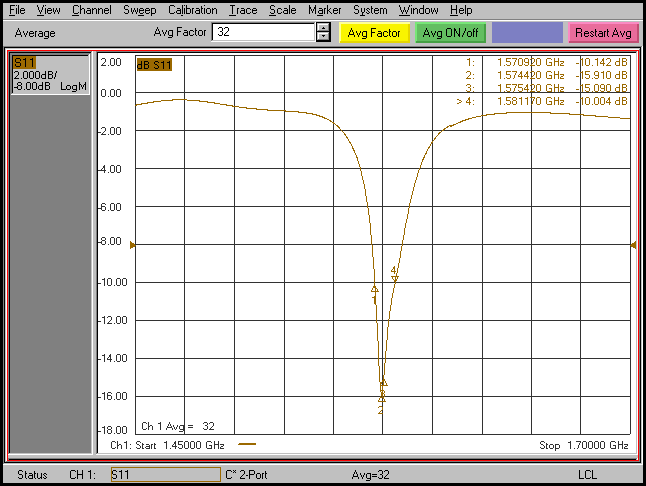
\includegraphics[width=\linewidth]{pictures/ant-s11.png}
        \caption{Paramètre S11 de l'antenne}
    \end{minipage}
    \hfill
    \begin{minipage}{0.45\textwidth}
        \centering
        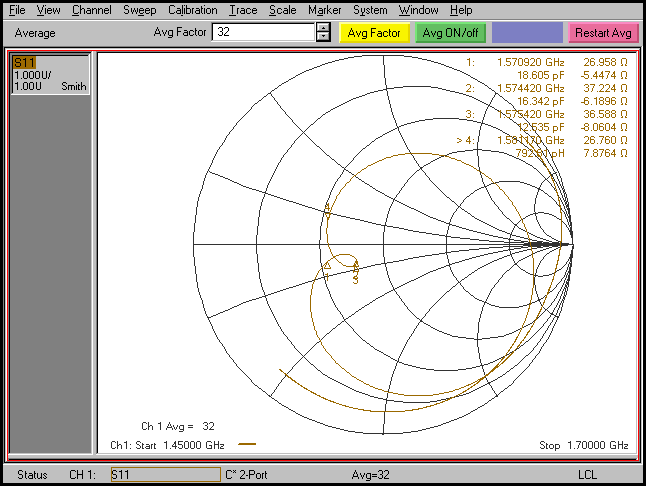
\includegraphics[width=\linewidth]{pictures/ant-smith.png}
        \caption{Smith Cart de l'antenne}
    \end{minipage}
\end{figure}


\subsection{PCB quelques points importants}
\subsubsection{Power Supply \& Dissipation Thermique}
	\subsubsection{Adaptation d'impédance}
	\subsubsection{Test points}
\end{document}











